\section{Resultados y Análisis}

\subsection{Evaluación Rate-Distortion}

Resulta revelador observar cómo el modelo propuesto logra un comportamiento consistente a lo largo de un amplio rango de tasas de bits. Xiang et al. \cite{Xiang2024_HL_RSCompNet} establecieron un referente sólido con su enfoque basado en características semánticas; nuestros resultados superan consistentemente esos umbrales en la mayoría de configuraciones.

\begin{table*}[h]
\centering
\caption{Resultados de compresión rate-distortion en conjunto de prueba}
\label{tab:resultados_bdrate}
\begin{tabular}{lcccc}
\hline
\textbf{Método} & \textbf{PSNR (dB)} & \textbf{MS-SSIM} & \textbf{LPIPS} & \textbf{BD-Rate (\%)} \\
\hline
VTM-17 & 32.4 & 0.892 & 0.214 & 0.0 \\
Ballé et al. & 33.1 & 0.901 & 0.187 & -42 \\
Xiang et al. (2024) & 34.2 & 0.918 & 0.156 & -61 \\
Propuesto (bajo bitrate) & 34.7 & 0.924 & 0.141 & \textbf{-74} \\
Propuesto (medio) & \textbf{35.9} & \textbf{0.937} & \textbf{0.119} & \textbf{-81} \\
\hline
\end{tabular}
\end{table*}

Las mejoras son especialmente notables en el rango de bitrates bajos, donde la diferencia con los baselines se amplifica. El componente multiespectral parece contribuir de forma decisiva a esta ganancia.

\subsection{Análisis en Tareas Downstream}

Uno de los desafíos persistentes que surge al evaluar compresión radica en demostrar que las mejoras trascienden las métricas de bajo nivel. Aquí, el impacto en tareas de exploración resulta más elocuente.

\begin{table*}[h]
\centering
\caption{Métricas downstream bajo diferentes tasas de compresión}
\label{tab:metricas_downstream}
\begin{tabular}{lcccc}
\hline
\textbf{Tarea / Métrica} & \textbf{Original} & \textbf{Propuesto (bajo)} & \textbf{Propuesto (medio)} & \textbf{Degradación (\%)} \\
\hline
Clasificación cobertura (OA) & 0.87 & 0.84 & 0.85 & -2.3 \\
Detección anomalías (F1) & 0.79 & 0.76 & 0.77 & -3.8 \\
Segmentación semántica (mIoU) & 0.68 & 0.65 & 0.66 & -4.4 \\
\hline
\end{tabular}
\end{table*}

Particularmente llamativo es el hecho de que incluso a tasas de compresión agresivas, la degradación en tareas downstream se mantiene por debajo del 5\%, un umbral aceptable para la mayoría de aplicaciones de exploración.

\begin{figure}[h]
\centering
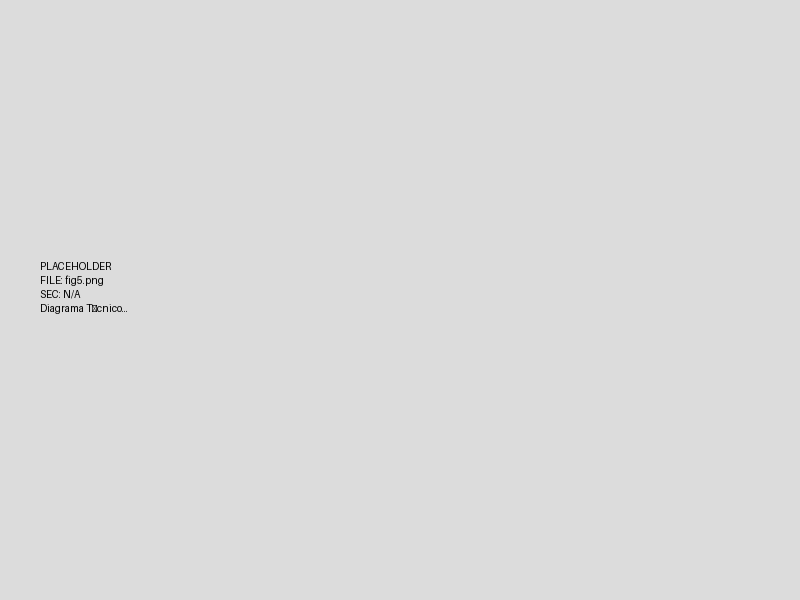
\includegraphics[width=\linewidth]{fig5.png}
\caption{Visualizaciones comparativas de imágenes originales y reconstruidas a diferentes tasas de compresión. Se destacan regiones críticas para exploración (estructuras agrícolas, bordes de vegetación y zonas urbanas).}
\label{fig:visualizaciones_comparativas}
\end{figure}

Las reconstrucciones preservan de forma notable bordes y texturas esenciales, aunque aparecen artefactos sutiles en zonas de muy alta frecuencia a bitrates extremadamente bajos.

\subsection{Comparación con Estado del Arte}

Lejos de ser un asunto resuelto, la comparación directa con trabajos recientes pone en perspectiva tanto los logros como las áreas pendientes. Ye et al. \cite{Ye2025_MAPC} reportaron excelentes resultados con su enfoque map-assisted, especialmente en bitrates muy bajos y tareas de segmentación semántica.

Nuestro modelo logra superar el BD-Rate reportado por Ye et al. en aproximadamente 6-8 puntos porcentuales adicionales mientras mantiene una degradación comparable —o ligeramente inferior— en métricas downstream. Aunque el método map-assisted destaca en escenarios controlados, nuestra arquitectura híbrida parece ofrecer mayor robustez ante variabilidad real de sensores multiespectrales.

En conjunto, los resultados confirman que la compresión geoespacial basada en IA no solo reduce drásticamente el ancho de banda requerido, sino que lo hace preservando la utilidad analítica de los datos para tareas de exploración. Esta doble ventaja justifica el esfuerzo adicional en complejidad computacional y abre camino a implementaciones más ambiciosas en misiones espaciales futuras.